\chapter{Introduction}
\label{Chap:Introduction}

\Ac{MRI} and \ac{MRS} measure signals from atomic nuclei. The most commonly used nucleus is the hydrogen nucleus ($^1$H) which consists of a positively charged proton. This is due to the fact that $^1$H is the most abundant nucleus in the human body, with an adult's bodyweight typically being made up of ~60\% water (H$_2$O) (more exact values can be estimated based on age, sex, height and weight \cite{Watson1980TotalMeasurements}). This means that tissues that have a larger H$_2$O concentration will generally have a stronger MR signal. In order to investigate, measure and quantify metabolism it is vitally important to be able to measure small differences in the products that are created due to metabolism (metabolites). Therefore, other reference nuclei are often used to investigate metabolism. In doing this it is important to choose a nucleus that is magnetically favourable and is found in metabolites that are of interest. Carbon-13 ($^{13}$C) \cite{Grist2019QuantifyingImaging,Brender2019DynamicHyperpolarization} and Phosphorous-31 ($^{31}$P) \cite{Gordon1980LocalizationResonance} are often used in research to quantify metabolite concentrations \textit{in vivo}. They have lower abundance in the human body (compared to $^1$H), but are quite magnetically favourable for MRS studies. Their abundances are usually too low for direct \ac{MRI} measurements, but the ability to separate different metabolites in each spectrum is important. Recently deuterium ($^2$H) has been shown to be a nucleus of interest when investigating metabolism in humans \textit{in vivo} \cite{Lu2017QuantitativeSpectroscopy,DeFeyter2018DeuteriumVivo}, and the field of deuterium MR has grown at a very fast rate thanks to its potential capabilities for investigating brain tumours \cite{DeFeyter2018DeuteriumVivo}, along with its relatively simple implementation.

\begin{figure}
    \centering
    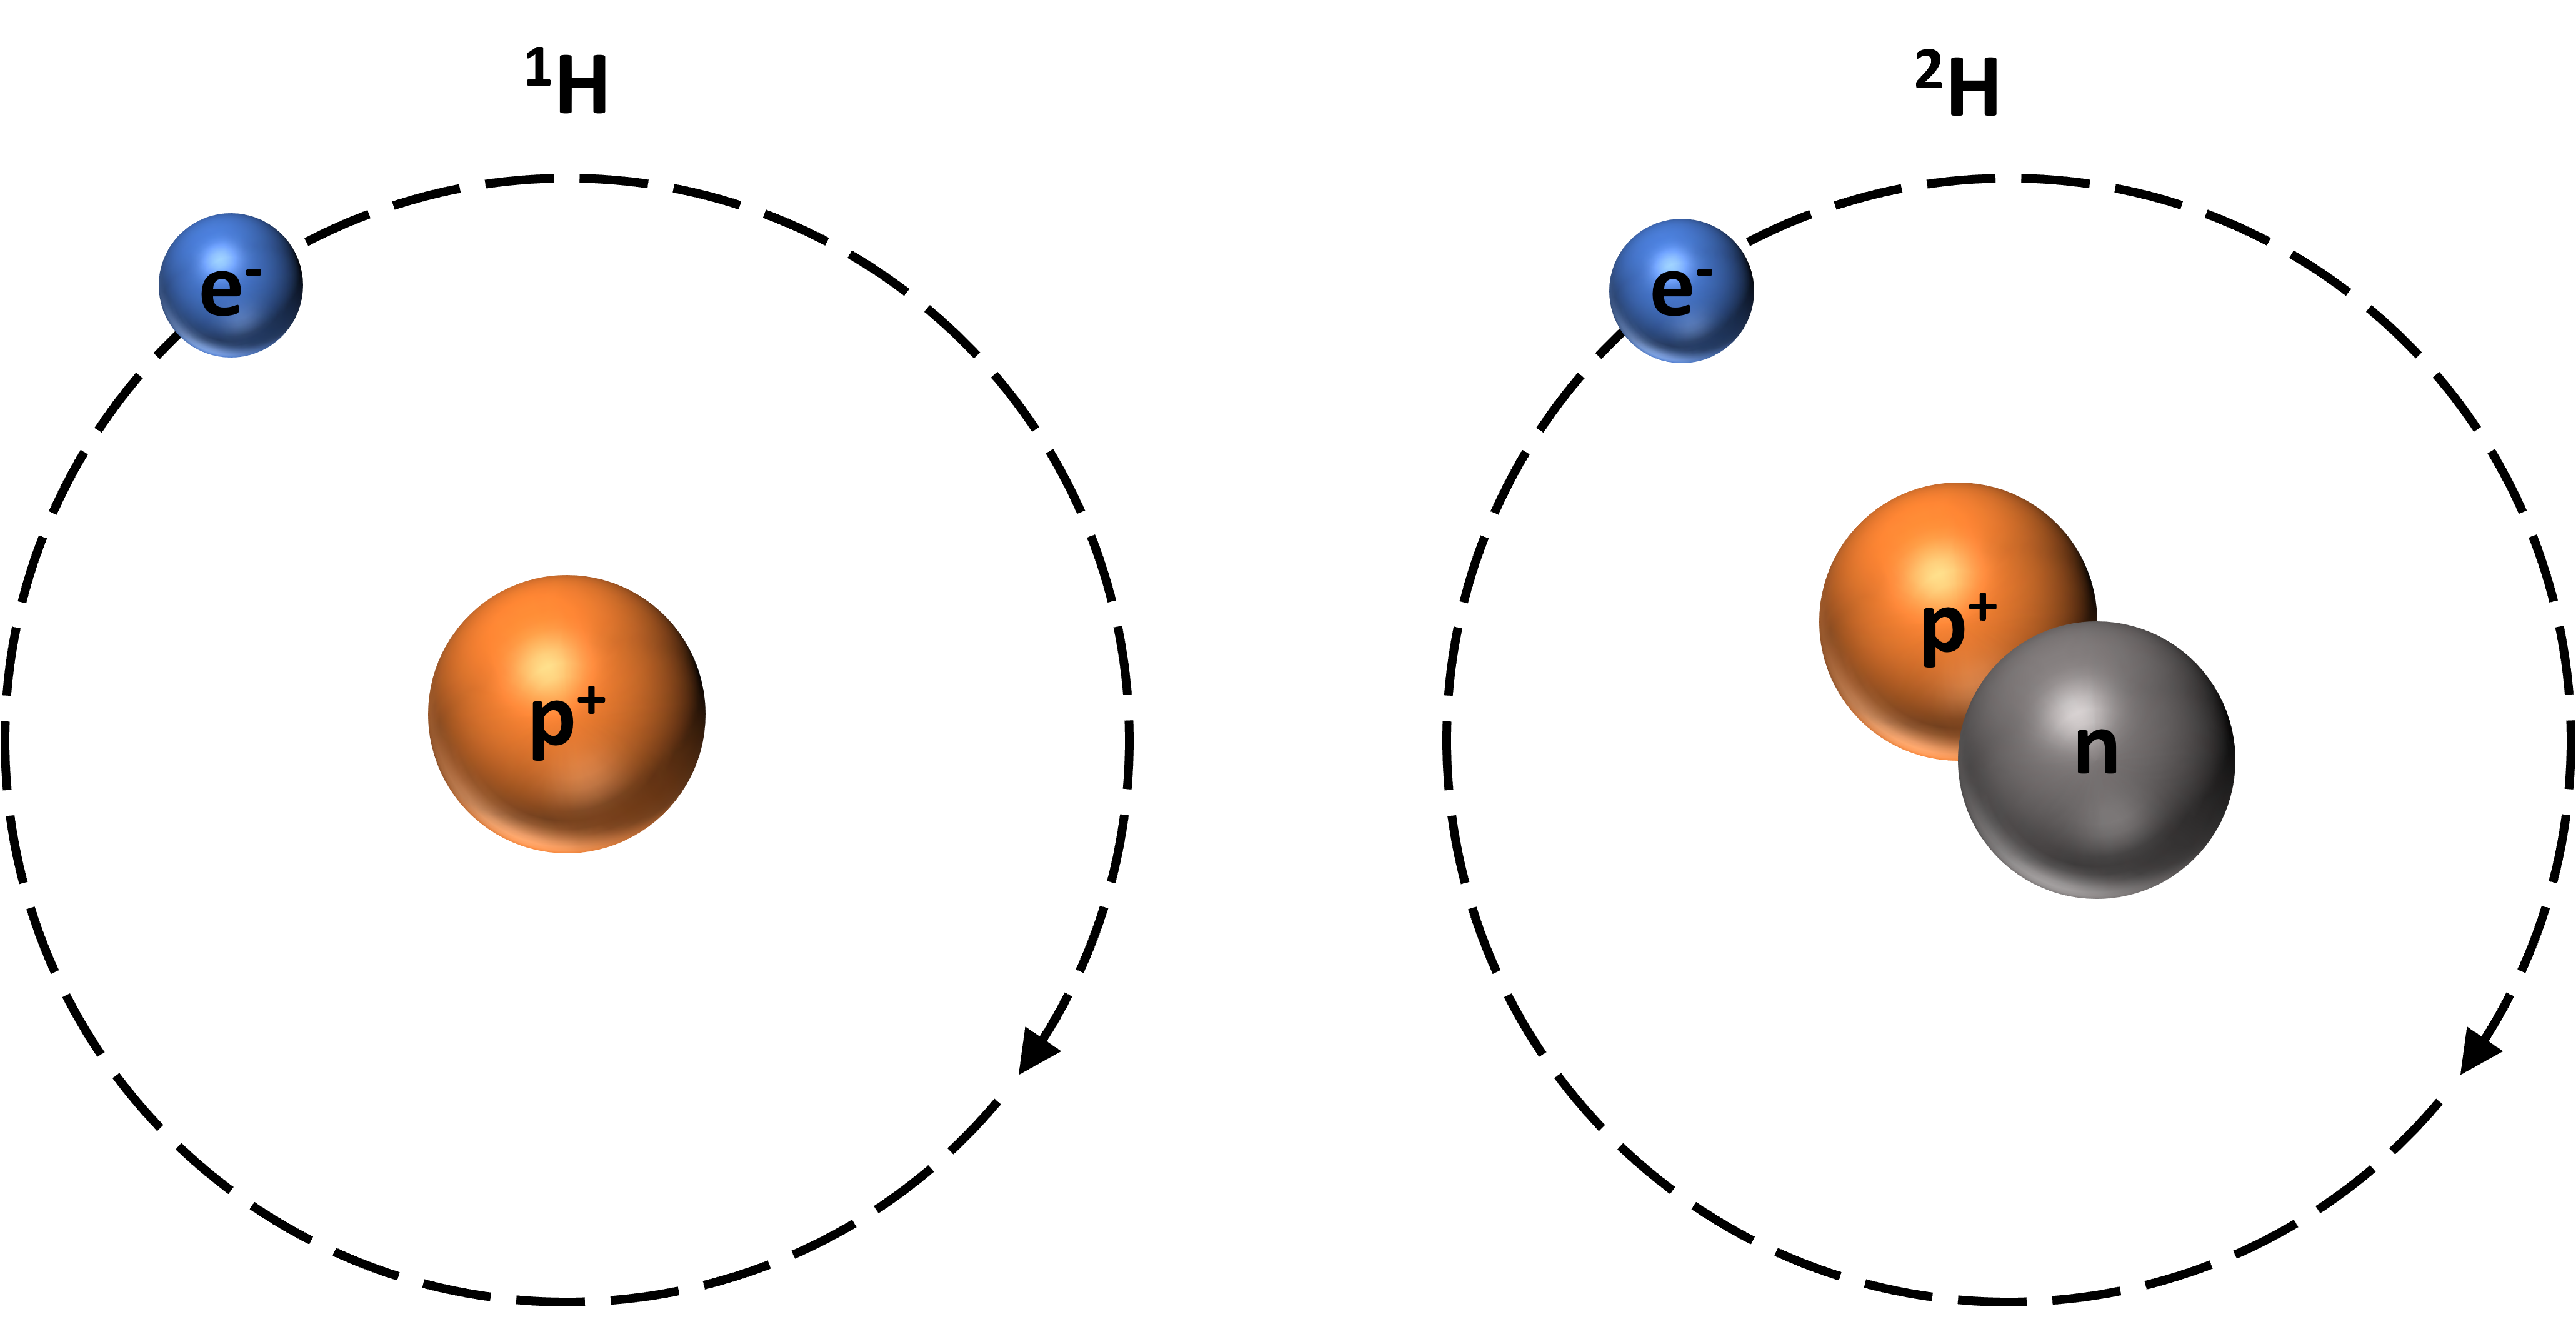
\includegraphics[width=0.9\textwidth]{Figures/Intro/1H2H.png}
    \caption{\textit{Schematic diagram of the atomic structure hydrogen ($^1$H, left) and deuterium atoms ($^2$H, right).}}
    \label{fig:intro:1H2H}
\end{figure}

\section{Metabolism}

Disrupted metabolism is a key aspect of many life-altering diseases including cancer and neurodegenerative diseases, such as \ac{AD}, \ac{PD} and \ac{MS} \cite{Gialleonardo2016TheImaging}. \ac{AD} has a European age-standardized prevalence of 4.4\% among people aged over 65 \cite{Qiu2009EpidemiologyIntervention}. One of the most prevalent and fatal metabolic diseases is cancer. In 2017 there were $\approx$375,000 new cancer cases in the UK \cite{CancerUK}, with $\approx$3\% of them being attributed to tumours in the brain and other parts of the CNS \cite{BrainUK}. The mortality rate of these cancers has remained significant and constant for the last decade \cite{BrainUK}. It is important therefore to develop tools for investigating metabolism \textit{in vivo}, and more specifically in brain tumours.

\begin{figure}
    \centering
    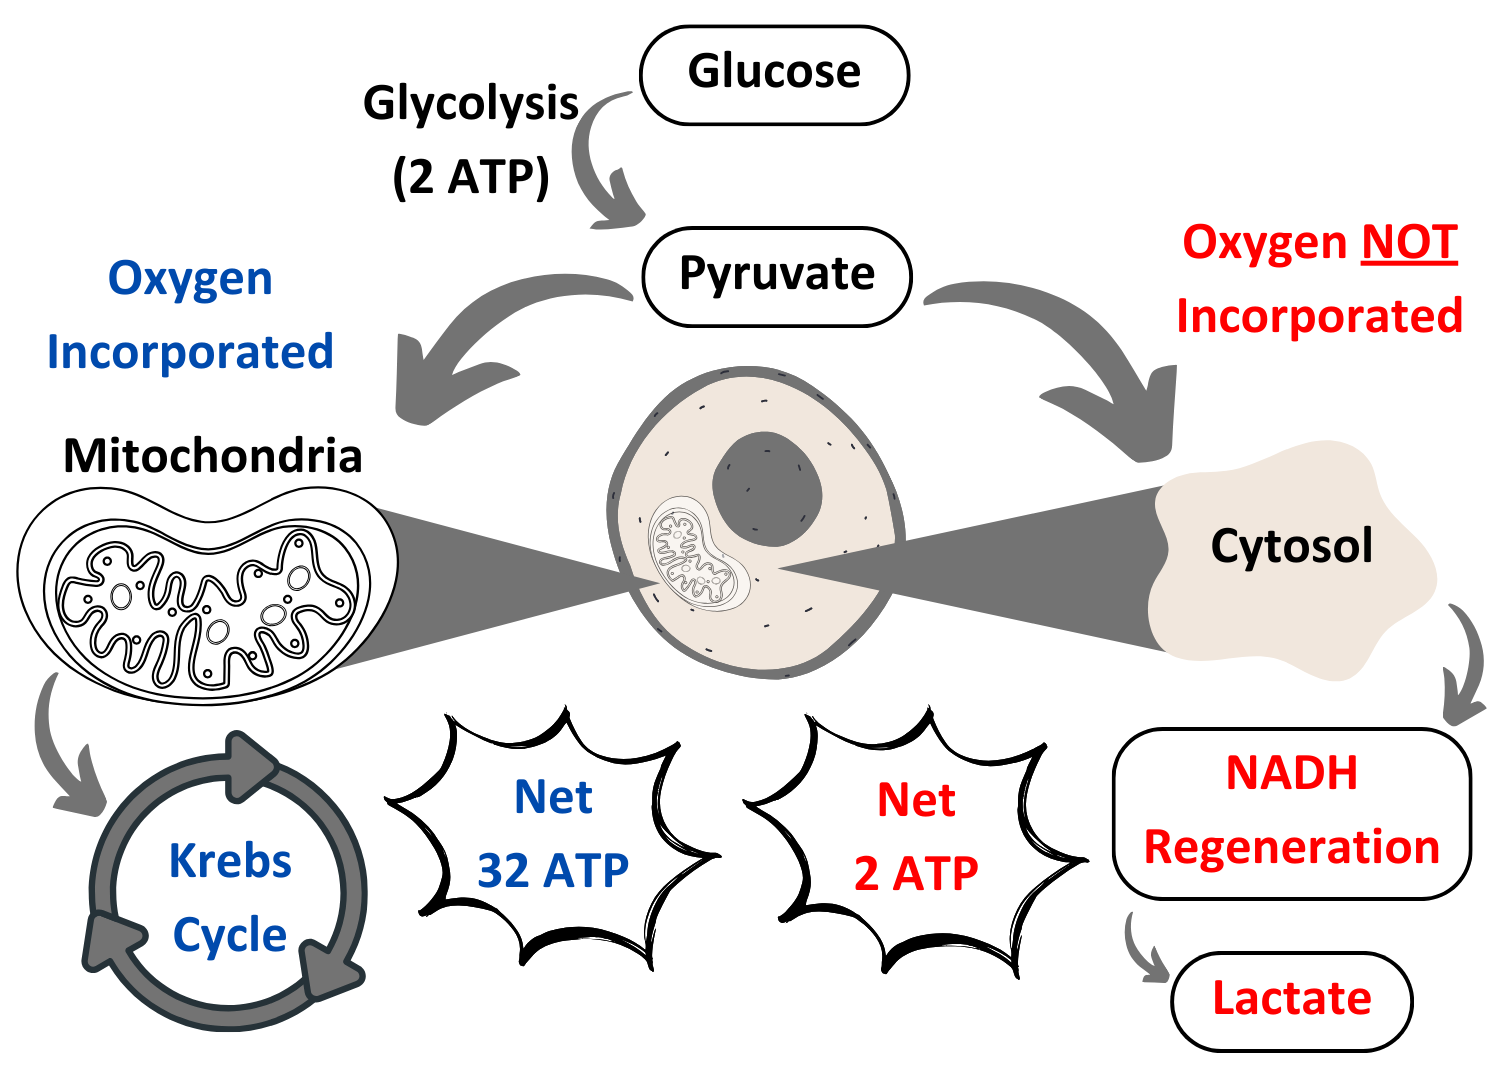
\includegraphics[width=0.75\textwidth]{Figures/Intro/Metabolism.png}
    \caption{\textit{Flow Chart demonstrating how glucose is metabolised into \ac{ATP} with (aerobic, blue) and without (anaerobic, red) oxygen being present. Healthy cells favour aerobic respiration whilst cancerous cells prefer anaerobic respiration.}}
    \label{fig:intro:Metabolism}
\end{figure}

Cancer is often considered to be a metabolic disease because as part of their growth, tumours affect and impair normal metabolism. The nucleic acid \ac{ATP} is used as energy currency in cells. In mammalian cells pyruvate is generated from glucose via glycolysis and produces two molecules of \ac{ATP} per each molecule of glucose. In healthy cells there are then two options for metabolism depending on the supply of oxygen to the cell, if oxygen is readily in supply a process called oxidative-phosphorylation takes place. Oxidative-phosphorylation is where pyruvate enters the mitochondria and enters the citric acid cycle, also known as the \ac{TCA} or Krebs cycle, where as many as thirty-two more \ac{ATP} are produced. This complete process is often referred to as aerobic respiration. The other option, when oxygen is not readily in supply, involves conversion of pyruvate into lactate in the cytosol of the cell through NADH regeneration. The complete process for the creation of lactate is known as lactic acid fermentation. Aerobic respiration is much more efficient in its energy production producing  around sixteen times more \ac{ATP} per mole of glucose compared to lactic acid fermentation \cite{Romero-Garcia2011TumorView}. 

\begin{figure}
    \centering
    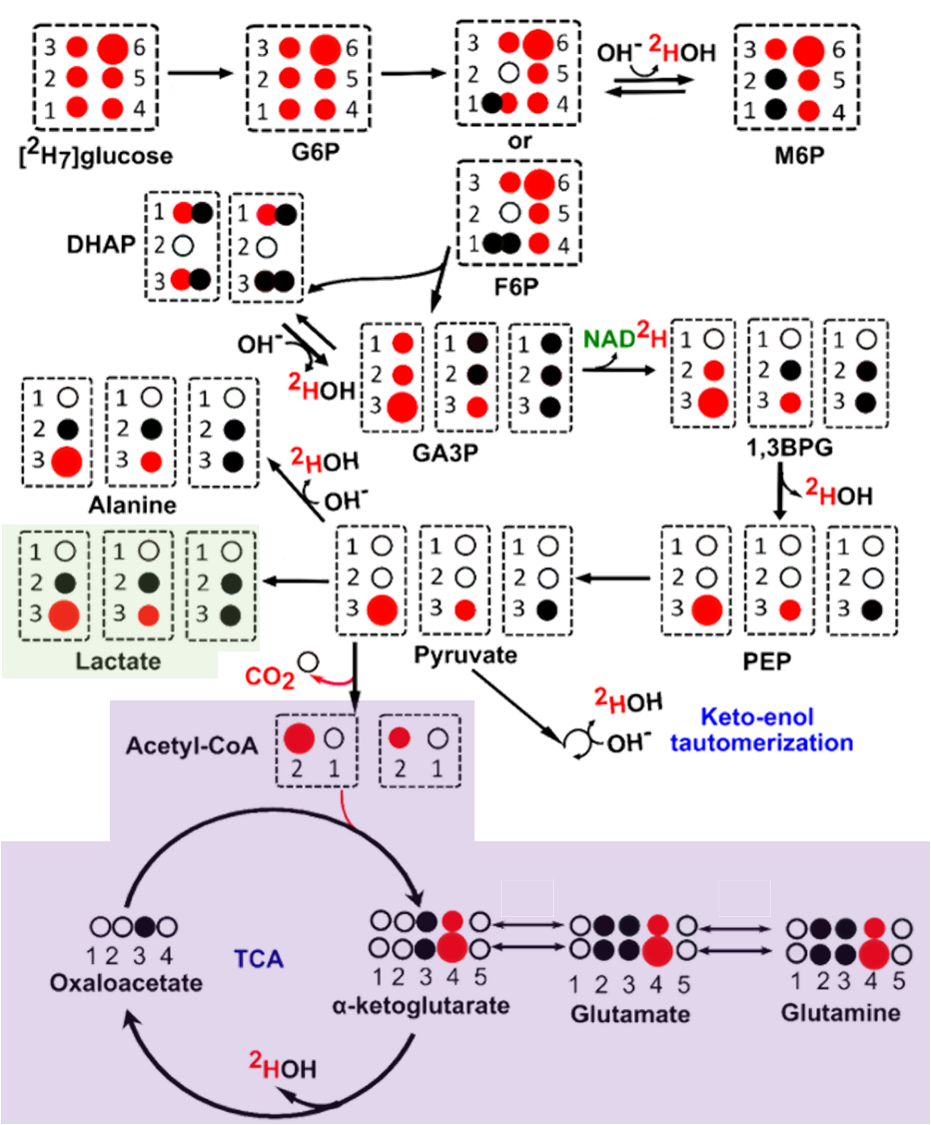
\includegraphics[width=0.9\textwidth]{Figures/Intro/D7_Metabolism.png}
    \caption{\textit{Metabolic pathway for $^2$H-labelled glucose, where all available sites for $^2$H labelling have been used. The small red circles represent individual $^2$H atoms, the large red circles represent two $^2$H atoms at the C6 and C6' sites. The black-filled and empty circles represent $^1$H and quarternary carbons, respectively. The \ac{TCA} cycle is labelled on the diagram, and the specific pathway for formation of glutamate and glutamine which results from oxidative phosphorylation, is highlighted in purple. The specific pathway for the formation on lactate resulting from lactic acid fermentation is highlighted in green. The glycolysis steps are shown from the glucose molecule to the pyruvate molecule. This figure is adapted from Figure 5 in \cite{Mahar2021DeuteratedGlucose}.}}
    \label{fig:intro:D7Metabolism}
\end{figure}

By replacing atoms found on a glucose molecule with atoms whose presence can be tracked, it is possible to track the metabolic products of the glucose molecule. If the replaced atoms make there way through metabolism into downstream metabolites such measurements it can therefore inform on the metabolic pathway taken. There are seven hydrogens (not including those in hydroxyl groups) in a glucose molecule which can be replaced with $^2$H atoms. During oxidative-phosphorylation, glutamate and glutamine are produced (the combination of the two is referred to as Glx) and of the seven hydrogen atoms only three are transferred to glutamine/glutamate. During lactic fermentation three of the hydrogen atoms are also transferred to lactate. These hydrogens come from the C1, C6 and C6' positions in the glucose molecule. The rest of the labels (C2, C3, C4 and C5) are lost in the production of water during lactic acid fermentation and aerobic respiration. The specific metabolic pathway undertaken after fully $^2$H-labelled glucose has been ingested is outlined in Fig. \ref{fig:intro:D7Metabolism}, which shows how each $^2$H label makes it way into downstream metabolites and also indicates where the $^2$H label can be lost. It is important to note that unlabelled lactate, glutamate and glutamine can be formed from deuterated metabolites in glycolysis and by multiple iterations of the \ac{TCA} cycle. All processes take place in the cell and the labelled glucose travels to the desired location in the blood vessels.

Otto Warburg observed in the \nth{20} century that tumours had a higher rate of glucose uptake \cite{WarburgBerlin-Dahlem1925TheCells,Warburg1956OnCells}. There were originally quite a few theories suggesting that cancerous cells had impaired mitochondria. It is now thought that the reason behind this effect is that cancerous cells are able to metabolise by either oxidative-phosphorylation or by fermentation regardless of how much oxygen is present to the cell. Lactic fermentation is favoured compared to oxidative-phosphorylation even though it is less energy/\ac{ATP} efficient. This leads to an increase in lactate and a decrease in Glx \cite{Romero-Garcia2011TumorView}.

\begin{figure}[ht]
    \centering
    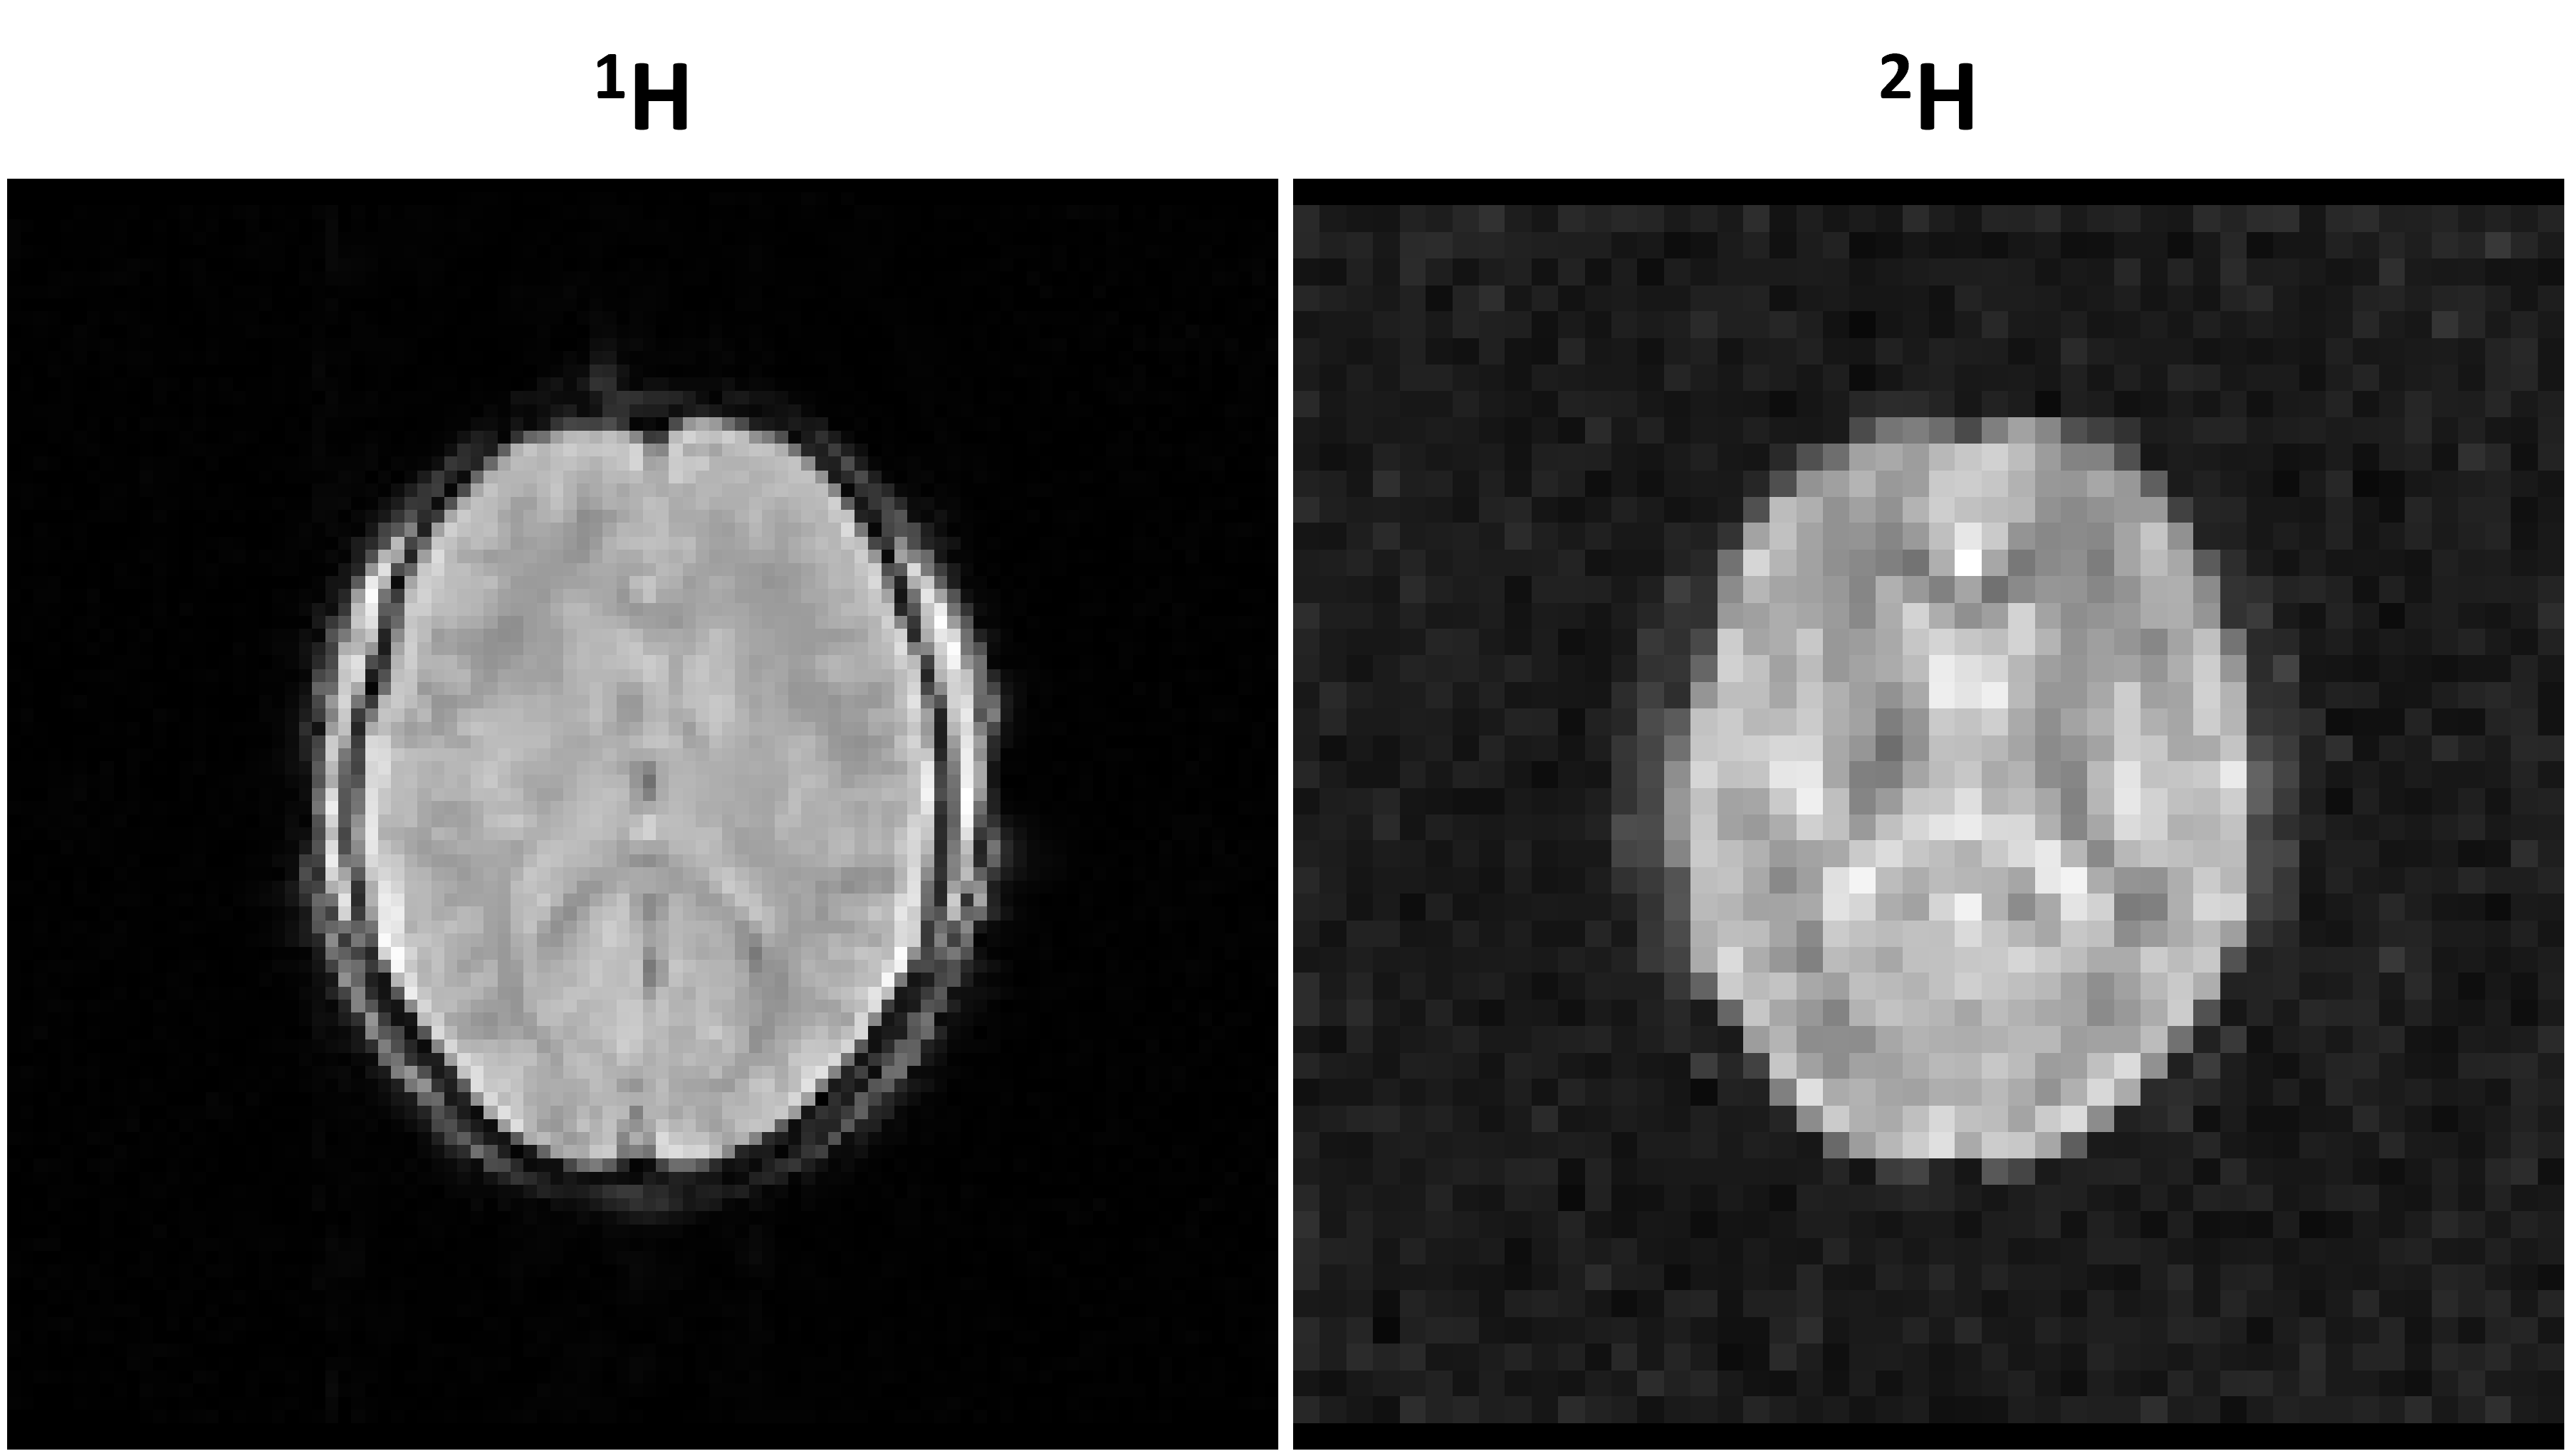
\includegraphics[width=0.9\textwidth]{Figures/Intro/1H2H_Brain.png}
    \caption{\textit{Images of the brain acquired using different nuclei, in the same scan session for the same participant using similar gradient echo sequences. Left is a $^1$H image with 3\textnormal{x}3\textnormal{x}2.5 mm$^3$ voxels acquired in 232 s. Right is a $^2$H image obtained with 6\textnormal{x}6\textnormal{x}10 mm$^3$ voxels with a scan duration of 354 s. It is important to note that the participant's $^2$H level is 100\textnormal{x} natural abundance as they have consumed heavy water (D$_2$O) as part of a study.}}
    \label{fig:intro:1H2H_Brain}
\end{figure}

Currently the most reliable way to accurately diagnose and monitor most cancers and metabolic diseases (such as \ac{AD} \cite{Shokouhi2014ImagingTomography} and \ac{PD} \cite{Meles2017MetabolicDisease}), in a non-invasive way, is by using \ac{PET} \cite{Almuhaideb201118F-FDGOncology}. Unfortunately this technique involves the use of a radioisotope inside the body which can put patients at further health risks, whilst a technique that is based on \ac{MRI} would be non-invasive and not require the use of ionising radiation. Cancerous cells have a much higher glucose uptake during metabolism than normal cells. This is the basis behind \ac{PET} imaging of cancer using $^{18}$F-labelled \ac{FDG}. Increased uptake of \ac{FDG} in a specific region gives an indication of the presence a cancerous tumour. \ac{FDG} \ac{PET} works by attaching a positron emitting atom to the glucose analog, \ac{FDG}. Once ingested it travels to the tissues where glucose is needed most. Inside cells the \ac{FDG} is phosphorylated but cannot undergo further metabolism, and so accumulates in metabolically active cells. When the $^{18}$F-label decays, the emitted positrons annihilate with electrons, creating two photons travelling in opposite directions. These photons can be detected giving information on the location of the glucose and therefore information as to where cancer is present. A limitation of \ac{FDG} \ac{PET} is that because it only detects the presence of $^{18}$F it doesn't provide information on any downstream metabolites. Since the brain is constantly metabolically active it can often be difficult to distinguish increases in metabolism compared to baseline, this is why it is important to choose a tracer with a low abundance. Metabolite signal/concentration maps from \ac{PET} are often displayed overlaid on high resolution anatomical images to provide accurate spatial distributions.

\begin{figure}
    \centering
    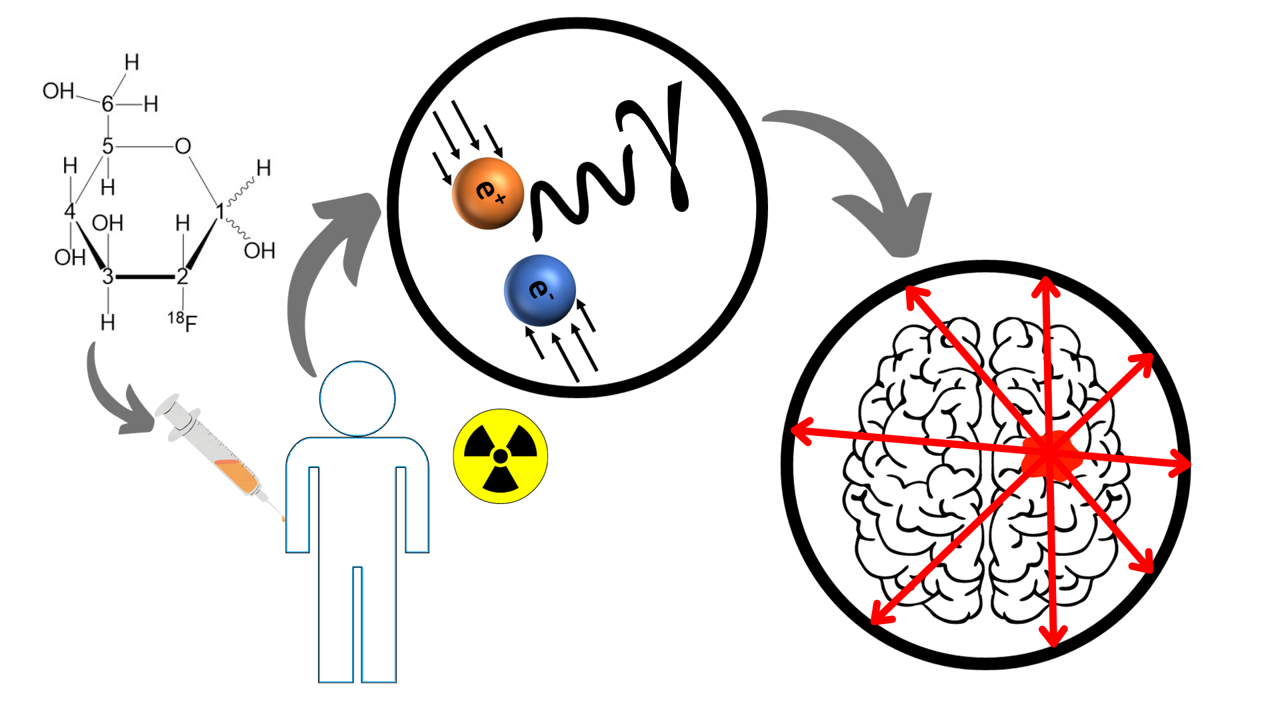
\includegraphics[width=1\textwidth]{Figures/Intro/PET_Scan.png}
    \caption{\textit{Diagram showing for \ac{PET} scanning works. Where the labelled glucose (left) is injected into participants/patients, and emitted positrons collide with electrons (middle). And how the resultant detected signals inform on areas of increased metabolism.}}
    \label{fig:intro:PET}
\end{figure}

\section{History of $^2$H Usage in Studying Metabolism}

\subsection{Pre-1980}

$^2$H was discovered in 1932 \cite{Urey1932AConcentration} from consideration of the apparent mass difference of hydrogen when measured chemically and with a mass spectrograph. It was rapidly realised that this stable isotope could be used to measure metabolism. Many papers were published demonstrating this \cite{Schoenheimer1935DeuteriumMetabolism,Schoenheimer1938TheMetabolism} for example via deuterating naturally occurring compounds such as fatty acids, feeding them to animals and then analysing the amount of deuterium found in bodily fluids. Shortly after this, the relaxation properties of $^2$H in \ac{NMR} were quantified in a solution of heavy water \cite{Bloembergen1948RelaxationAbsorption}. One possible explanation as to why it then took so long for this technique combined with \ac{NMR} to become popular is due to the rising interest (at the time) \cite{DeFeyter2021DeuteriumFuture} in use of radioactive isotopes $^3$H \cite{Thompson1953StudiesRat} and $^{14}$C \cite{Turteltaub1990AcceleratorDNA.} for metabolic studies. The health concerns around use of radioactive isotopes led to a resurgence of $^2$H metabolism research in the 1980's.

\subsection{1980 to the 21\textsuperscript{st} Century}

% Graphs of fat lipid changes from paper or from our own NA work 

\begin{figure}
    \centering
    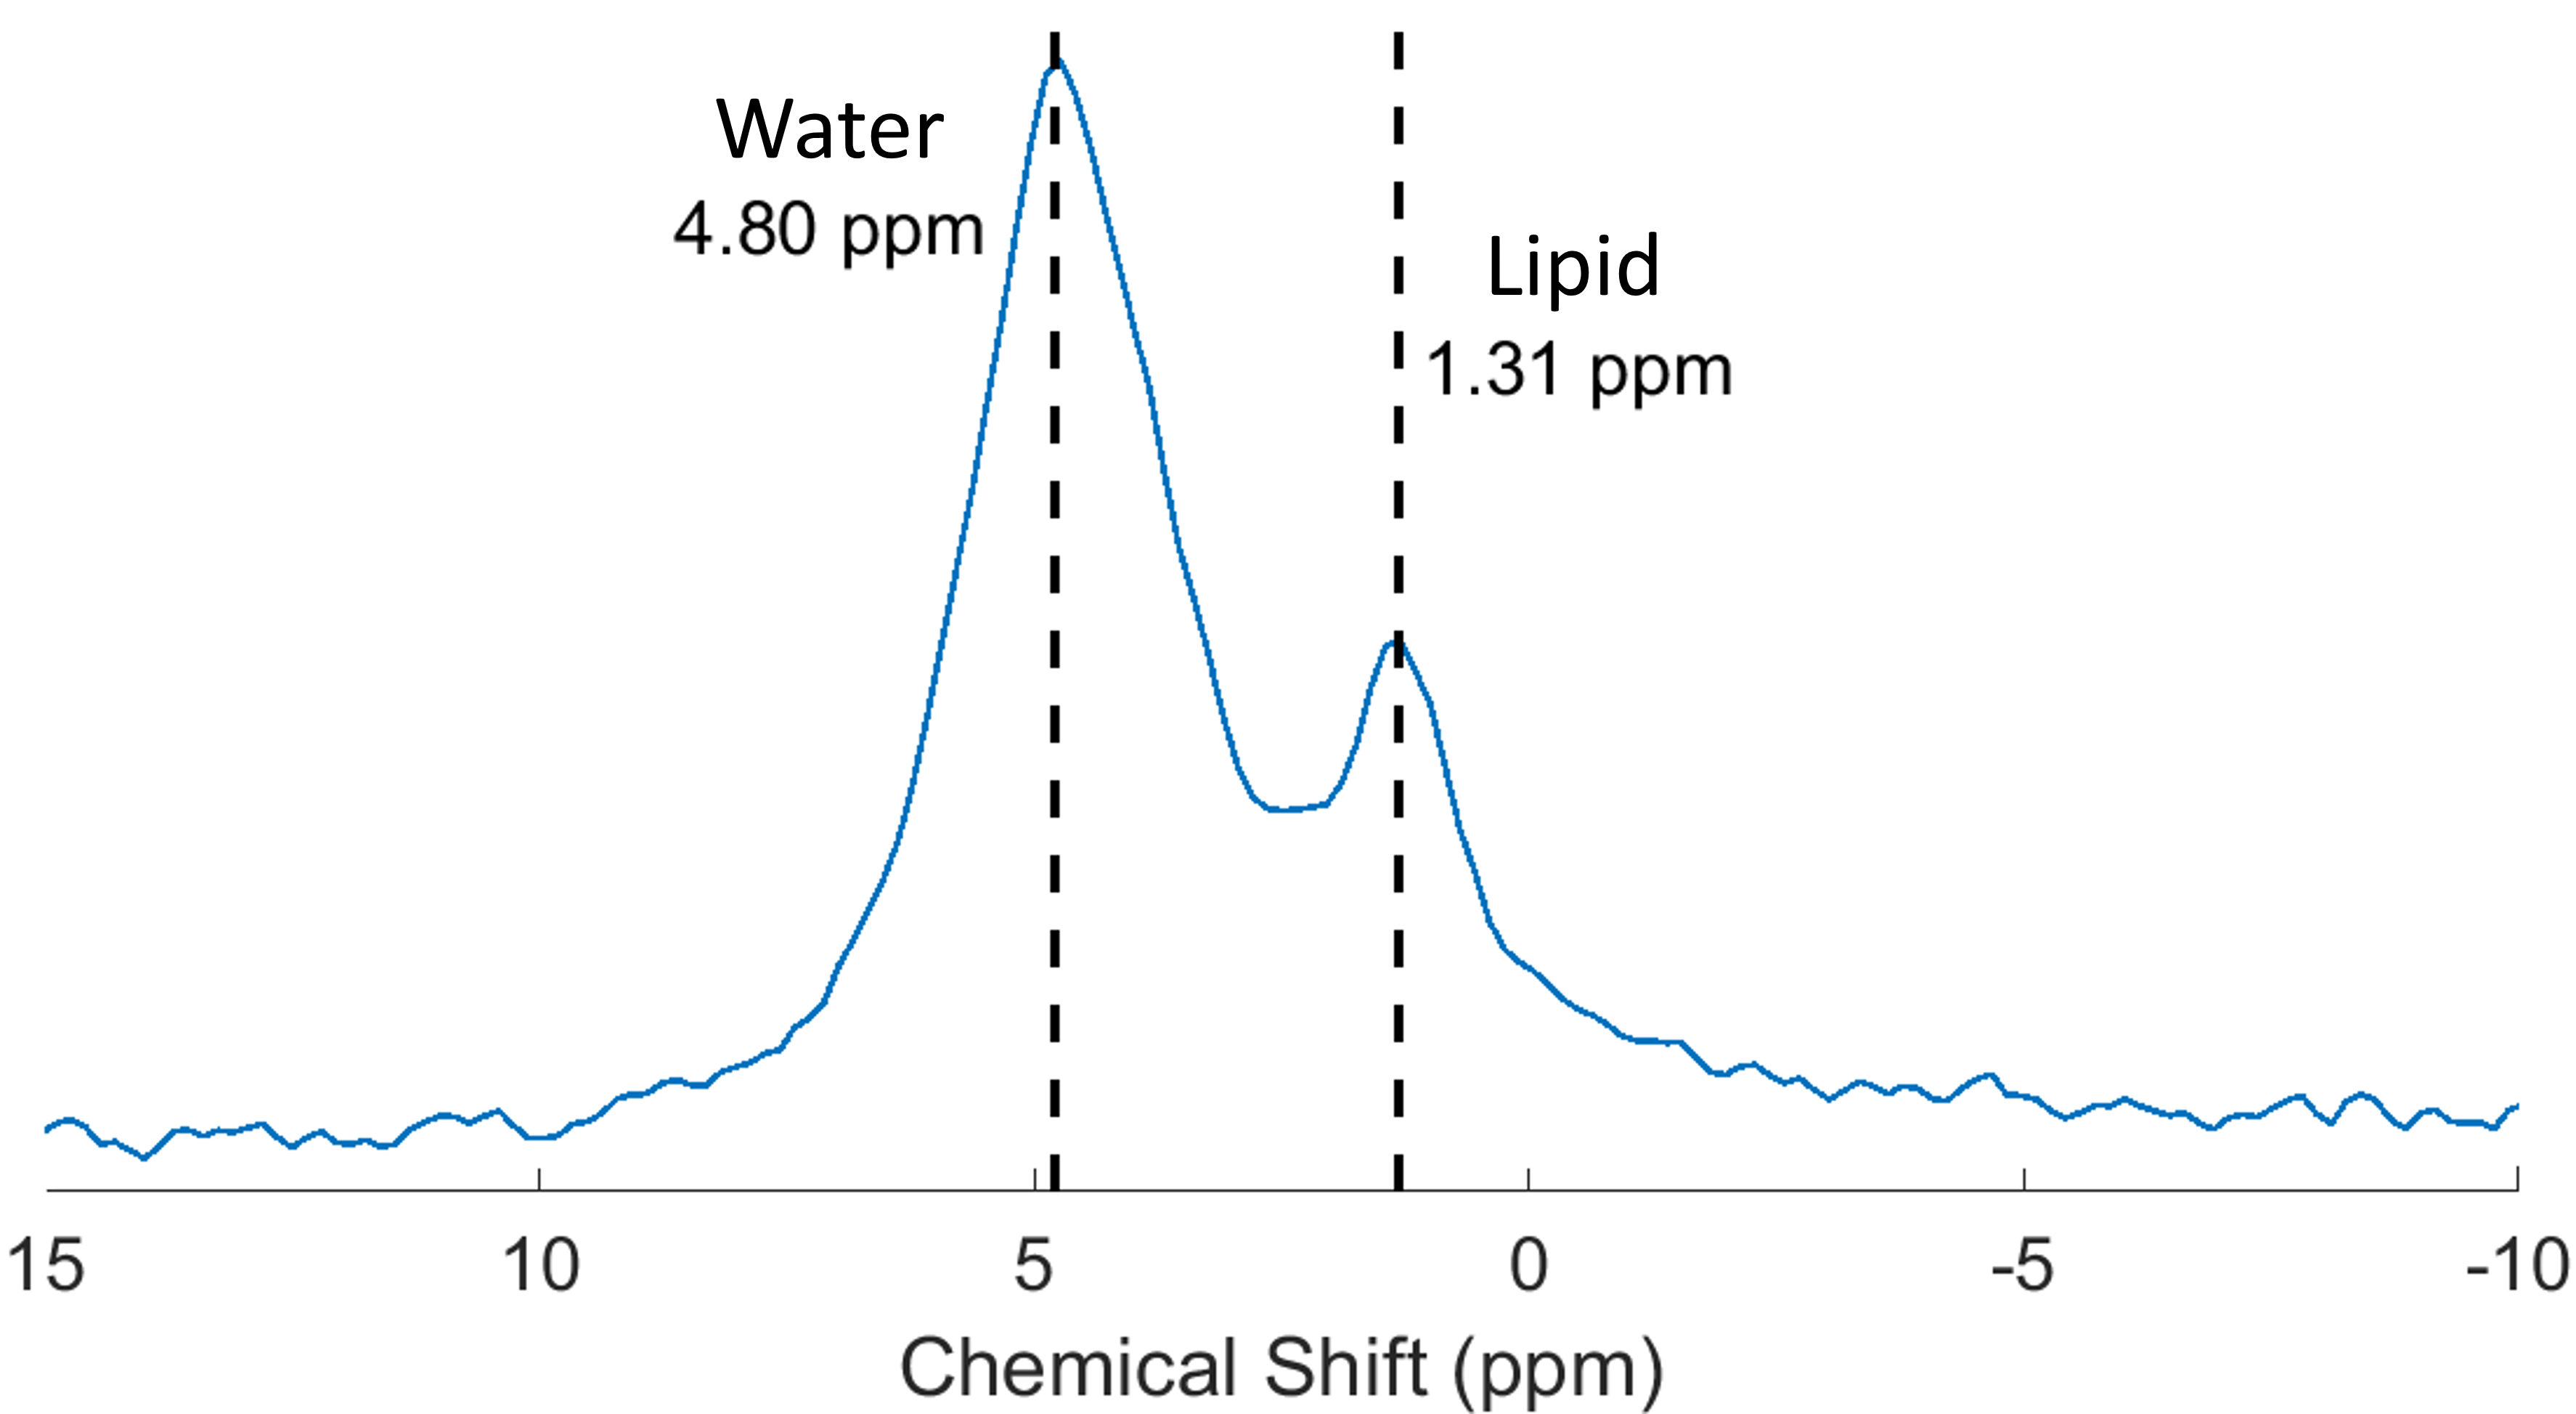
\includegraphics[width=0.8\textwidth]{Figures/Intro/NA_Spectra.png}
    \caption{\textit{Non-localised $^2$H spectra obtained from the calf \textit{in vivo} showing signals from water at a chemical shift of 4.8 ppm and fat/lipid signals at 1.3 ppm.}}
    \label{fig:intro:NA}
\end{figure}

The first \textit{in vivo} $^2$H NMR study was performed in 1986 \cite{Brereton1986PreliminarySpectroscopy} in mice. \Ac{D$_2$O} ingestion was used to increase $^2$H abundance, and an increase in fat/lipid signal was measured. Shortly after this, numerous pre-clinical studies were published that involved using heavy water as a tracer, looking at: the brain \cite{Ewy1988DeuteriumSitu}, blood flow and perfusion \cite{Ackerman1987DeuteriumTracer.} and iron stores \cite{Irving1987InSpectroscopy}. Other deuterated compounds then started to be used such as labelled choline \cite{Eng1990RenalStudy}, with the first instance of deuterated glucose being used being in 1986 \cite{Barrow1986NMRMobilis}. This started a trend of other studies using deuterated glucose to investigate bacterial metabolism \cite{Aguayo1988HighMetabolism.} and liver gycogen synthesis \cite{Goodman1989UseSynthesis}. All the aforementioned studies involved animal models. The number of studies that involved $^2$H then slowed down before a long hiatus. One potential reason for this hiatus was the success' of \textit{in vivo} $^1$H \cite{Harada1984IdentificationScience}, $^{13}$C \cite{Cohen1980UseLiver} and $^{31}$P \cite{Sappey-Marinier1992EffectSpectroscopy} measurements. However, there has recently been a resurgence in $^2$H MR research and more specifically its use in studying metabolism.

\subsection{The Last Seven Years}

\begin{figure}[H]
    \centering
    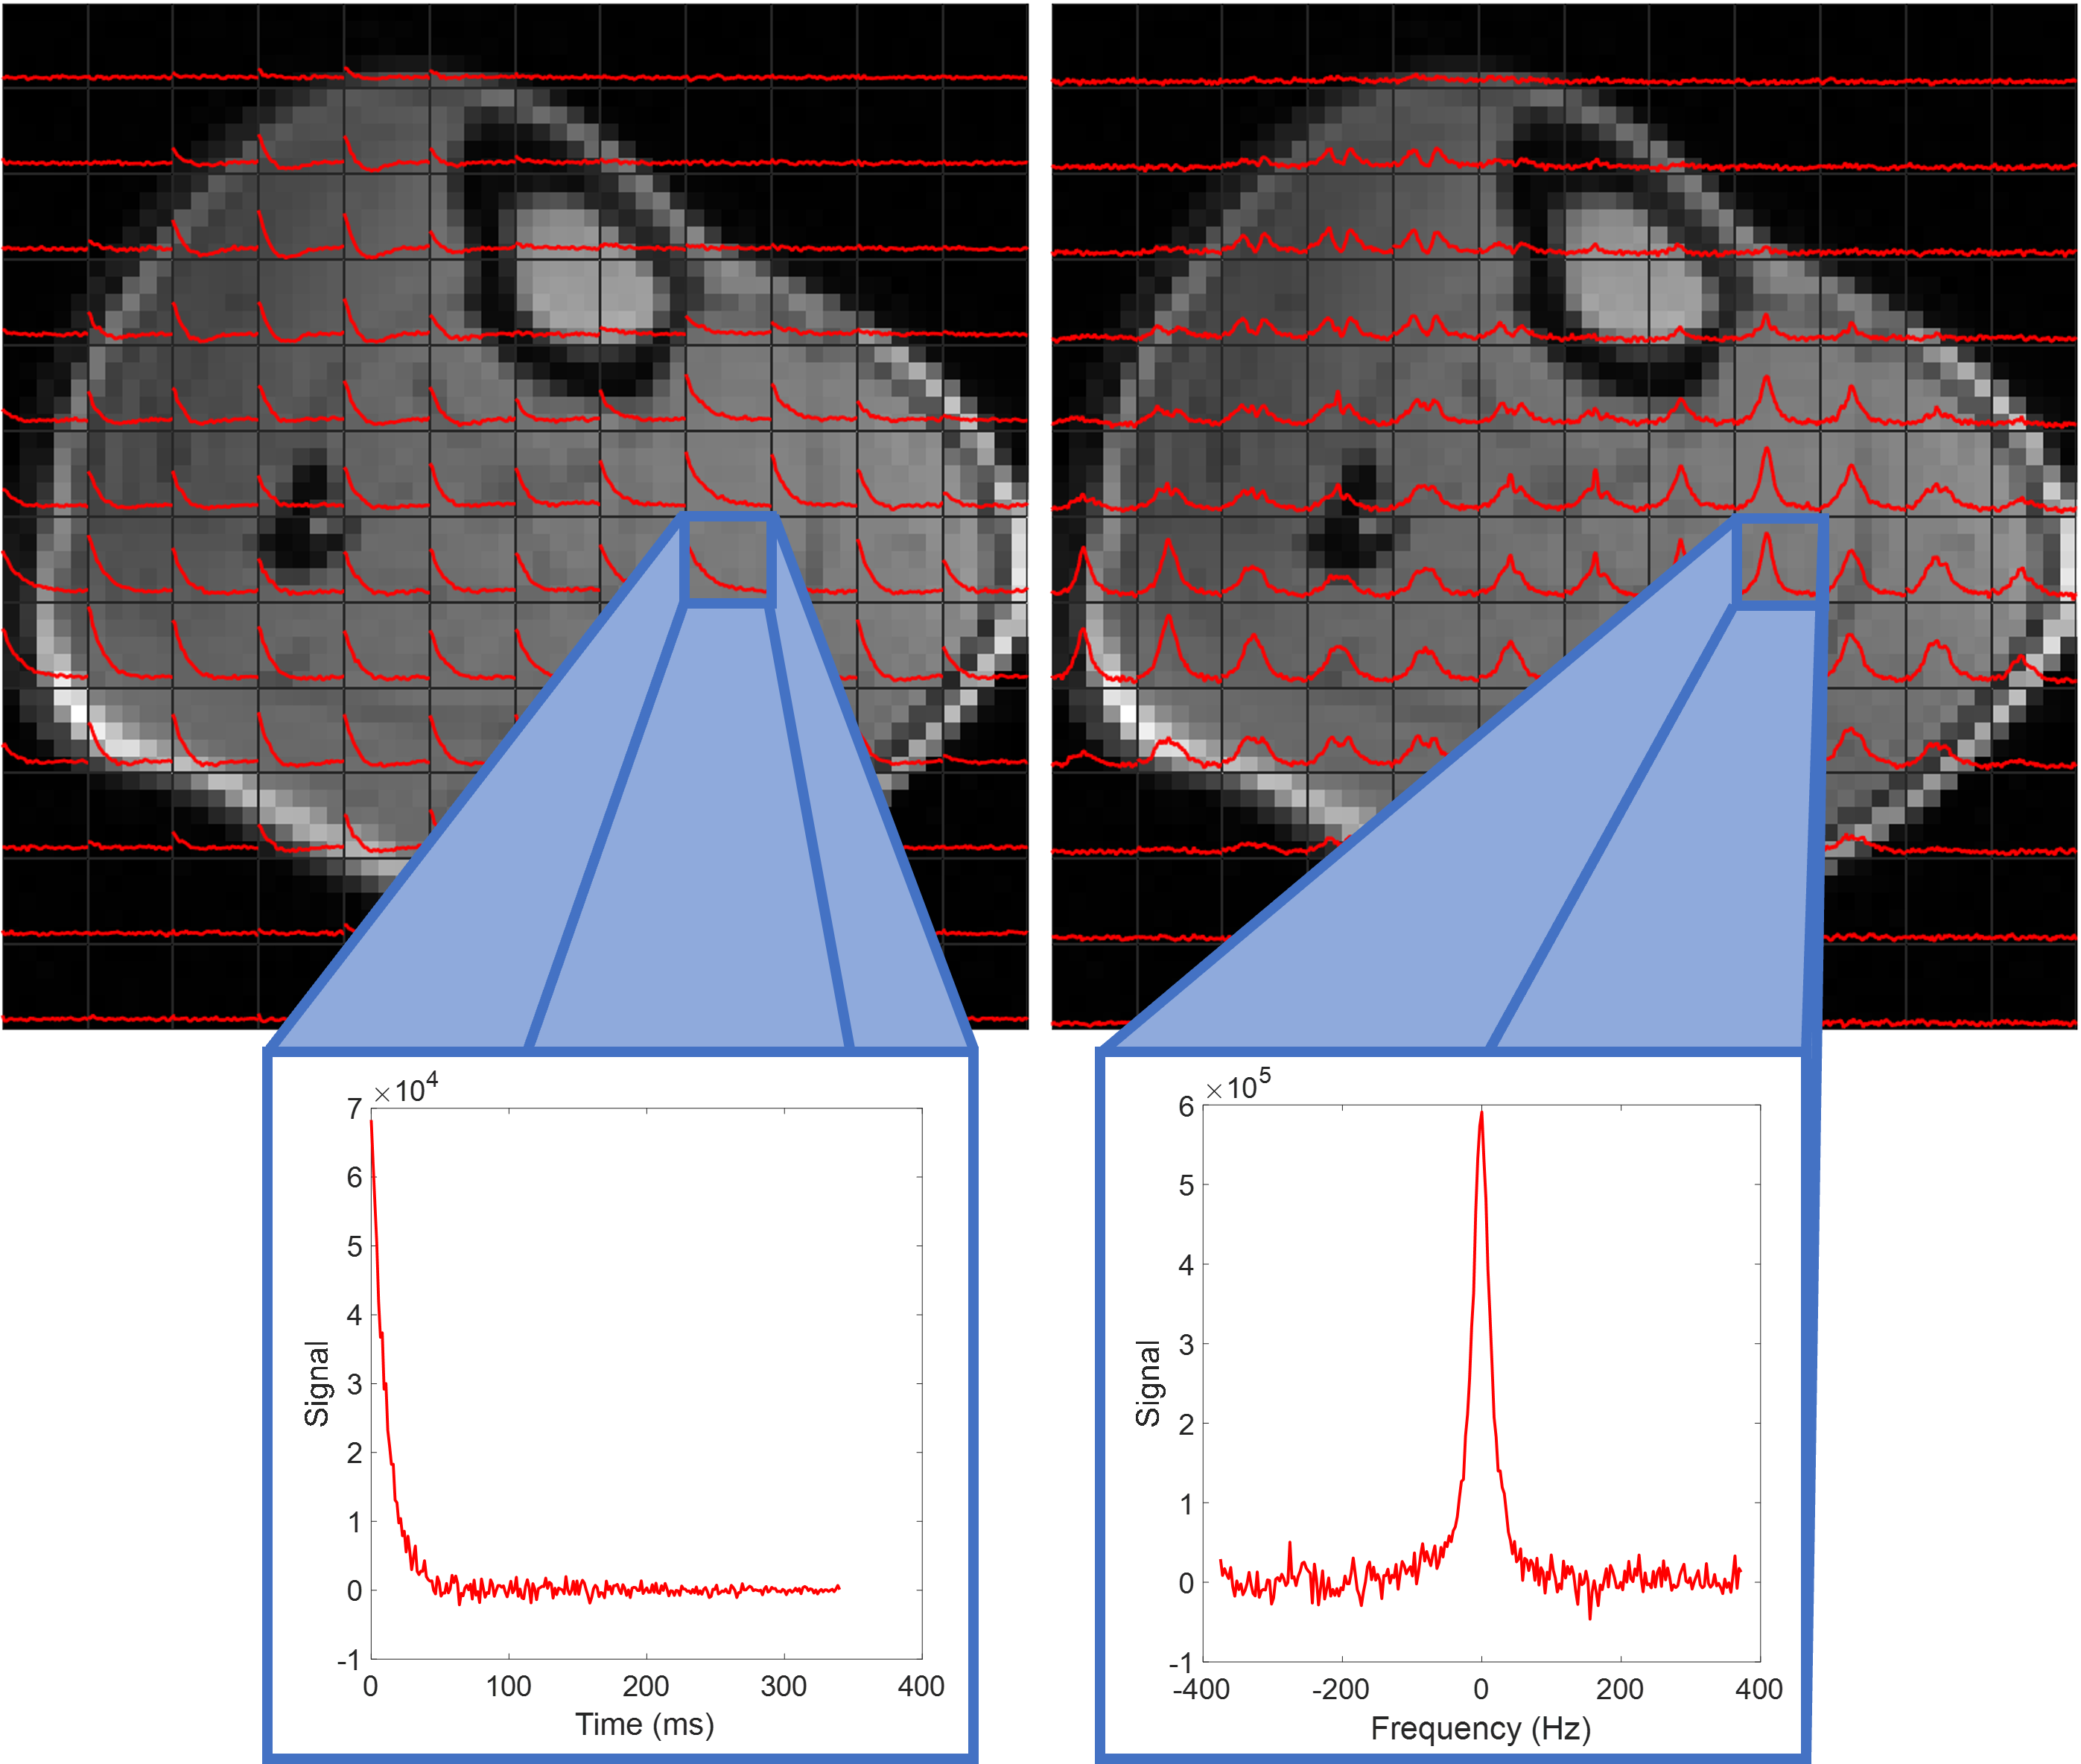
\includegraphics[width=0.8\textwidth]{Figures/Intro/CSI.png}
    \caption{\textit{Example \ac{NA} \ac{MRSI} data overlayed onto an anatomical image of the calf. The left shows the localised \ac{FID} data from voxels with one voxel blown up. The right shows the corresponding localised spectroscopic data (Fourier transform of the \ac{FID} shown on the left) with data from one voxel blown up.}}
    \label{fig:intro:CSI}
\end{figure}

[6,6'-$^2$H$_2$] (also known as $^2$H$_2$-glucose or D$_2$-glucose) was first used in an \textit{in vivo} MR study in an animal model \cite{Lu2017QuantitativeSpectroscopy} in 2017, where both the $^1$H atoms at C6 and C6' are replaced with $^2$H. And soon after this technique was applied \textit{in vivo} in humans, where it was demonstrated that differences between normal and tumour tissue could be seen in maps of $^2$H signals from downstream metabolic products of the labelled glucose \cite{DeFeyter2018DeuteriumVivo}. This form of glucose is currently the most commonly used deuterated tracer in research \cite{DeFeyter2018DeuteriumVivo,DeFeyter2021DeuteriumFuture,Ruhm2022Dynamic9.4T,Roig2022Deuterium7T,deGraaf2020OnImaging}. At \ac{NA} only a deuterated water (HDO) peak/signal is visible in a typical spectrum, because the noise level is higher than the $^2$H signals from other $^2$H in other molecules. After ingestion of D$_2$-glucose, peaks from deuterated glucose (Glu), a combination of glutamine and glutamate (Glx) and lactate (Lac) appear. \ac{CSI} or other \ac{MRSI} methods, can be used to produce maps of each of these metabolites. Production of maps of the ratio of the Glx and Lac concentration have been shown to provide a good delineation of cancerous tissue \cite{DeFeyter2018DeuteriumVivo,Straathof2021DeuteriumBrain}. Other deuterated compounds have been used to measure different metabolic pathways. These include [$^2$H$_3$]-acetate (D$_3$-acetate) \cite{DeFeyter2018DeuteriumVivo,Rich20201HVivo}, [6,6'-$^2$H$_2$]-fructose (D$_2$-fructose) \cite{Zhang202366-2H2Cancer}, as well as other forms of deuterated glucose. For example [2,3,4,6,6'-$^2$H$_5$] (D$_5$-glucose) \cite{Zou2023AImaging} has recently been found to be cheaper to produce than D$_2$-glucose.

% De Feyter images or CSI images

\section{Aims}

The aims of the work described in this thesis are to develop $^2$H \ac{MRI} and \ac{MRSI} scanning at the \ac{SPMIC} at the University of Nottingham at both clinical high field (3T) and ultra-high field (7T). Work outlined in this thesis is relevant for the implementation of $^2$H at a range of field strengths. The more specific primary aim of the work described in this thesis is to set the ground for scanning patients with brain tumours using DMI at 7T.

All the work that is outlined in this thesis involves the use of $^2$H \ac{MRI} and \ac{MRSI} techniques and includes: measuring the relaxation times of \ac{HDO} in different healthy \textit{in vivo} brain tissues; assessing the increase in $^2$H abundance as \Ac{D$_2$O} is ingested in different healthy \textit{in vivo} brain tissues; using different amounts of $^2$H labelling of glucose to assess \textit{in vivo} metabolism in the brain of healthy participants; evaluating whether the ingestion of \Ac{D$_2$O} in conjunction with $^2$H MR can be used to investigate lipid turnover and using $^2$H MR following ingestion of \Ac{D$_2$O} to assess the quadrupolar \ac{HDO} splitting in anisotropic and isotropic tissues using regular \ac{MRI} and \ac{MRSI}, as well as double-quantum-filtered \ac{MRI} and MRSI.

\section{Description of Work}

Chapter two covers the theory underlying the work that was undertaken in this thesis. This includes the theory behind \ac{MRI} and \ac{MRSI} and more specifically the difference between $^1$H and $^2$H \ac{NMR} including magnetisation, relaxation and pulse sequences. This chapter also describes the extra hardware adaptations that are needed for $^2$H signal detection, ranging from amplifiers to \ac{RF} coil construction.

Chapter three reports the first measurements of $^2$H signals from the brain in subjects who had ingested heavy water. A \ac{D$_2$O} ingestion routine is outlined, as well as a scanning routine undertaken to allow the quantification of $^2$H relaxation times in the human brain using \ac{MEGE} scans with different \ac{TR}-values. Similar scans were then also used for some participants to track the $^2$H increase that occurs immediately following the ingestion of \ac{D$_2$O}. It was shown that the $^2$H increase from \ac{MRI}/\ac{MRS} follows what is expected from blood sampling, and the relaxation times for different tissues are reported with statistical significance shown.

% Chapter four gives an overview of some of the research that has been conducted so far in deuterium metabolic imaging (DMI) predicts the potential benefits of using D$_7$-glucose as opposed to D$_2$-glucose. 

Chapter four describes the first measurements of metabolism in human subjects using \ac{DMI} with D$_7$-glucose. The methodology used so healthy participants can ingest deuterated glucose is outlined as well as the scanning routine with parameters for CSI scanning. Increases in signal levels for all downstream metabolites resulting from the D$_7$-glucose were found, suggesting that better \ac{CNR} between healthy and tumour tissue would be possible, despite the more complicated analysis.

Chapter five describes the importance of measuring lipid turnover and the limitations of the present methodology involving heavy-water loading and biopsy, and suggests a new routine that uses $^2$H \ac{MRI}/\ac{MRS} instead. A new routine of ingesting \ac{D$_2$O} is given as well as 
 a regular scanning routine that is repeated once a fortnight. Increases in $^2$H lipid signal were detected, but new advances/improvements are needed to make this technique is clinically viable.

Chapter six describes an investigation of the quadrupolar splitting seen in the $^2$H signal from water in muscle, where the orientation of the muscle relative the external magnetic field affects the splitting amplitude. After participants have their $^2$H abundance increased by ingesting \ac{D$_2$O}, \ac{MRSI} and \ac{DQF} \ac{MRSI} has been used to show the relationship between the anisotropy and quadrupolar interaction in the forearm and the calf.

Finally, chapter seven brings together all the work that has been conducted in this thesis, and gives direction on any future work that may follow from it.